\documentclass[conference,twocolumn]{IEEEtran}
\usepackage{blindtext}
\usepackage[utf8]{inputenc} 
\usepackage{cmap}
\usepackage[T1]{fontenc}

\usepackage[german]{babel}
\usepackage[babel,german=quotes,german=guillemets]{csquotes}
%\selectlanguage{ngerman}
%\documentclass[conference]{../sty/IEEEtran}

%\usepackage{ifpdf}

%\ifpdf
%pdf code
%\else
%dvi code
%\fi

% \ifCLASSINFOpdf conditional that works the same way.

% *** CITATION PACKAGES ***
%
% \usepackage{cite}
% cite.sty was written by Donald Arseneau
% V1.6 and later of IEEEtran pre-defines the format of the cite.sty package
% \cite{} output to follow that of IEEE. Loading the cite package will
% result in citation numbers being automatically sorted and properly
% "compressed/ranged". e.g., [1], [9], [2], [7], [5], [6] without using
% cite.sty will become [1], [2], [5]--[7], [9] using cite.sty. cite.sty's
% \cite will automatically add leading space, if needed. Use cite.sty's
% noadjust option (cite.sty V3.8 and later) if you want to turn this off.
% cite.sty is already installed on most LaTeX systems. Be sure and use
% version 4.0 (2003-05-27) and later if using hyperref.sty. cite.sty does
% not currently provide for hyperlinked citations.
% The latest version can be obtained at:
% http://www.ctan.org/tex-archive/macros/latex/contrib/cite/
% The documentation is contained in the cite.sty file itself.

% *** GRAPHICS RELATED PACKAGES ***
%
%\ifCLASSINFOpdf
  \usepackage[pdftex]{graphicx}
  \graphicspath{{/img/}}
  \DeclareGraphicsExtensions{.pdf,.jpeg,.png}
%\else
%  \usepackage[dvips]{graphicx}
%  \graphicspath{{/img/}}
%  \DeclareGraphicsExtensions{.eps}
%\fi

% *** MATH PACKAGES ***
%
\usepackage[cmex10]{amsmath}

\interdisplaylinepenalty=2500

% *** SPECIALIZED LIST PACKAGES ***
%
%\usepackage{algorithmic}
% algorithmic.sty was written by Peter Williams and Rogerio Brito.
% This package provides an algorithmic environment fo describing algorithms.
% You can use the algorithmic environment in-text or within a figure
% environment to provide for a floating algorithm. Do NOT use the algorithm
% floating environment provided by algorithm.sty (by the same authors) or
% algorithm2e.sty (by Christophe Fiorio) as IEEE does not use dedicated
% algorithm float types and packages that provide these will not provide
% correct IEEE style captions. The latest version and documentation of
% algorithmic.sty can be obtained at:
% http://www.ctan.org/tex-archive/macros/latex/contrib/algorithms/
% There is also a support site at:
% http://algorithms.berlios.de/index.html
% Also of interest may be the (relatively newer and more customizable)
% algorithmicx.sty package by Szasz Janos:
% http://www.ctan.org/tex-archive/macros/latex/contrib/algorithmicx/


% *** ALIGNMENT PACKAGES ***
%
\usepackage{array}

\usepackage{mdwmath}
\usepackage{mdwtab}

\usepackage{eqparbox}
% Also of notable interest is Scott Pakin's eqparbox package for creating
% (automatically sized) equal width boxes - aka "natural width parboxes".
% Available at:
% http://www.ctan.org/tex-archive/macros/latex/contrib/eqparbox/





% *** SUBFIGURE PACKAGES ***
%\usepackage[tight,footnotesize]{subfigure}
% subfigure.sty was written by Steven Douglas Cochran. This package makes it
% easy to put subfigures in your figures. e.g., "Figure 1a and 1b". For IEEE
% work, it is a good idea to load it with the tight package option to reduce
% the amount of white space around the subfigures. subfigure.sty is already
% installed on most LaTeX systems. The latest version and documentation can
% be obtained at:
% http://www.ctan.org/tex-archive/obsolete/macros/latex/contrib/subfigure/
% subfigure.sty has been superceeded by subfig.sty.


%\usepackage[caption=false]{caption}
%\usepackage[font=footnotesize]{subfig}
% subfig.sty, also written by Steven Douglas Cochran, is the modern
% replacement for subfigure.sty. However, subfig.sty requires and
% automatically loads Axel Sommerfeldt's caption.sty which will override
% IEEEtran.cls handling of captions and this will result in nonIEEE style
% figure/table captions. To prevent this problem, be sure and preload
% caption.sty with its "caption=false" package option. This is will preserve
% IEEEtran.cls handing of captions. Version 1.3 (2005/06/28) and later 
% (recommended due to many improvements over 1.2) of subfig.sty supports
% the caption=false option directly:
%\usepackage[caption=false,font=footnotesize]{subfig}
%
% The latest version and documentation can be obtained at:
% http://www.ctan.org/tex-archive/macros/latex/contrib/subfig/
% The latest version and documentation of caption.sty can be obtained at:
% http://www.ctan.org/tex-archive/macros/latex/contrib/caption/


% *** FLOAT PACKAGES ***
%
%\usepackage{fixltx2e}
% fixltx2e, the successor to the earlier fix2col.sty, was written by
% Frank Mittelbach and David Carlisle. This package corrects a few problems
% in the LaTeX2e kernel, the most notable of which is that in current
% LaTeX2e releases, the ordering of single and double column floats is not
% guaranteed to be preserved. Thus, an unpatched LaTeX2e can allow a
% single column figure to be placed prior to an earlier double column
% figure. The latest version and documentation can be found at:
% http://www.ctan.org/tex-archive/macros/latex/base/

%\usepackage{stfloats}
% stfloats.sty was written by Sigitas Tolusis. This package gives LaTeX2e
% the ability to do double column floats at the bottom of the page as well
% as the top. (e.g., "\begin{figure*}[!b]" is not normally possible in
% LaTeX2e). It also provides a command:
%\fnbelowfloat
% to enable the placement of footnotes below bottom floats (the standard
% LaTeX2e kernel puts them above bottom floats). This is an invasive package
% which rewrites many portions of the LaTeX2e float routines. It may not work
% with other packages that modify the LaTeX2e float routines. The latest
% version and documentation can be obtained at:
% http://www.ctan.org/tex-archive/macros/latex/contrib/sttools/
% Documentation is contained in the stfloats.sty comments as well as in the
% presfull.pdf file. Do not use the stfloats baselinefloat ability as IEEE
% does not allow \baselineskip to stretch. Authors submitting work to the
% IEEE should note that IEEE rarely uses double column equations and
% that authors should try to avoid such use. Do not be tempted to use the
% cuted.sty or midfloat.sty packages (also by Sigitas Tolusis) as IEEE does
% not format its papers in such ways.


% *** PDF, URL AND HYPERLINK PACKAGES ***
%
\usepackage{url}
% url.sty was written by Donald Arseneau. It provides better support for
% handling and breaking URLs. url.sty is already installed on most LaTeX
% systems. The latest version can be obtained at:
% http://www.ctan.org/tex-archive/macros/latex/contrib/misc/
% Read the url.sty source comments for usage information. Basically,
% \url{my_url_here}.

% correct bad hyphenation here
\hyphenation{op-tical net-works semi-conduc-tor}

% Bib
%\bibliographystyle{IEEEtran}

\usepackage[%
 backend=biber,%
 style=numeric,%
% bibstyle=alphabetic,%
% citestyle=alphabetic,%
 natbib=true,%
 sorting=anyt,%
 sortcites=true,%
 hyperref=auto,%
 maxnames=3,%
 minnames=1,%
]{biblatex}

\bibliography{bibo.bib}

\newcommand{\longpage}{\enlargethispage{\baselineskip}}
\newcommand{\verylongpage}{\enlargethispage{2\baselineskip}}
\newcommand{\shortpage}{\enlargethispage{-\baselineskip}}
\newcommand{\veryshortpage}{\enlargethispage{-2\baselineskip}}
\newcommand{\x}[1]{\mathrm{#1}}

%\newcommand{\pmsm}{permanentmagneterregten Synchronmaschine}
%\newcommand{\FOR}{feldorientierte Regelung}
%\newcommand{\pwm}{Pulsweitenmodulation}

\begin{document}

\title{Ansätze zur Parameteridentifikation einer PMSM}

\author{\IEEEauthorblockN{Benjamin Ternes, IEEE Member}
\IEEEauthorblockA{Hochschule Bochum\\
Fachbereich Elektrotechnik und Informatik\\
Bochum, Germany\\
E-mail: benjamin.ternes@hs-bochum.de\\
GitHub: \url{https://github.com/benjiternes/}}
\and
\IEEEauthorblockN{Jan Feldkamp}
\IEEEauthorblockA{Hochschule Bochum\\
Fachbereich Elektrotechnik und Informatik\\
Bochum, Germany\\
E-mail: jan.feldkamp@hs-bochum.de}}
%\and
%\IEEEauthorblockN{James Kirk\\ and Montgomery Scott}
%\IEEEauthorblockA{Starfleet Academy\\
%San Francisco, California 96678-2391\\
%Telephone: (800) 555--1212\\
%Fax: (888) 555--1212}}

% conference papers do not typically use \thanks and this command
% is locked out in conference mode. If really needed, such as for
% the acknowledgment of grants, issue a \IEEEoverridecommandlockouts
% after \documentclass

% for over three affiliations, or if they all won't fit within the width
% of the page, use this alternative format:
% 
%\author{\IEEEauthorblockN{Michael Shell\IEEEauthorrefmark{1},
%Homer Simpson\IEEEauthorrefmark{2},
%James Kirk\IEEEauthorrefmark{3}, 
%Montgomery Scott\IEEEauthorrefmark{3} and
%Eldon Tyrell\IEEEauthorrefmark{4}}
%\IEEEauthorblockA{\IEEEauthorrefmark{1}School of Electrical and Computer Engineering\\
%Georgia Institute of Technology,
%Atlanta, Georgia 30332--0250\\ Email: see http://www.michaelshell.org/contact.html}
%\IEEEauthorblockA{\IEEEauthorrefmark{2}Twentieth Century Fox, Springfield, USA\\
%Email: homer@thesimpsons.com}
%\IEEEauthorblockA{\IEEEauthorrefmark{3}Starfleet Academy, San Francisco, California 96678-2391\\
%Telephone: (800) 555--1212, Fax: (888) 555--1212}
%\IEEEauthorblockA{\IEEEauthorrefmark{4}Tyrell Inc., 123 Replicant Street, Los Angeles, California 90210--4321}}

% use for special paper notices
%\IEEEspecialpapernotice{(Invited Paper)}

\maketitle

\begin{abstract}
\boldmath
Diese Veröffentlichung setzt sich mit den Problemen und Ansätzen der Parameteridentifikation bei permanentmagneterregten Synchronmaschinen auseinander.
Da eine Realisierung an Messverfahren aus zeitlichen Gründen nicht möglich ist, sollen theoretische und industrietaugliche Verfahren aus aktuellen Veröffentlichungen gegenübergestellt werden.
Anhand einer ausführlichen Literaturrecherche sollen Ansätze zur Identifikation der Induktivitäten, des Ständerwiderstandes und der Permanentmagnetflussverkettung erarbeitet werden.
Außerdem soll kurz auf die Berücksichtigung der Eisenverluste eingegangen werden, da diese erhebliche Auswirkungen auf die bestimmten Parameter haben.
Abschließend werden die Auswirkungen der Parameterfehler erläutert.
\end{abstract}

\begin{IEEEkeywords}
permanentmagneterregte Synchronmaschine, Identifikation, Induktivitäten, Statorwiderstand, Eisenverluste, Parameterfehler
\end{IEEEkeywords}


% For peer review papers, you can put extra information on the cover
% page as needed:
% \ifCLASSOPTIONpeerreview
% \begin{center} \bfseries EDICS Category: 3-BBND \end{center}
% \fi
%
% For peerreview papers, this IEEEtran command inserts a page break and
% creates the second title. It will be ignored for other modes.
\IEEEpeerreviewmaketitle

%\tableofcontents

\section{Einleitung}
Synchronmaschinen mit Permanentmagneterregung werden in vielen Anwendungen eingesetzt.
Oftmals sind dies Anwendungen, die eine hochdynamische Regelung erfordern.
Aus Kosten- und Wartungsgründen wird oft auf einen Drehgeber verzichtet, die Lage wird dann \enquote{geberlos} aus den identifizierten Größen berechnet.
Die hochdynamischen \enquote{geberlosen} Regelungen benötigen die Induktivitäten der Maschine nicht nur als konstante Größen, sondern abhängig von den momentanen Strömen \autocite{Kellner2012}.
Die Flussverkettung der Permanentmagnete ändert sich aufgrund von Alterungserscheinungen und Temperaturveränderungen im Laufe des Betriebs.
Der ohmsche Ständerwiderstand, der sich durch Erwärmung des Ständers im Laufe des Betriebs verdoppeln kann, wird zur Drehmomentberechnung benötigt.
%Induktivitäten können auf verschiedene Arten gemessen werden.
Induktivitäten können auf verschiedene Arten offline gemessen werden.
Eine Möglichkeit ist die Nutzung der im Rahmen der Maschinenauslegung durchgeführten Finite-Elemente-Berechnung (FEM).
Die Herausforderung hierbei ist, dass die auf Basis einer vereinfachten und idealisierten Maschine durchgeführte FEM-Berechnung dennoch realistische Werte liefern soll.
%Im Rahmen der Maschinenauslegung durchgeführten Finite-Elemente-Methode zur Berechnung der Induktivitäten entstehen in einem vereinfachten Modell (zweidimensional), dass dennoch realistische Werte liefern soll.
Bei realen Maschinen treten Fertigungstoleranzen auf und zum anderen werden die Wickelköpfe der Maschinen in der FEM-Berechnung nicht berücksichtigt \autocite{ternes2012}.
%Aus diesen Gründen ist es sinnvoll, die Induktivitäten offline und an der realen Maschine zu messen.
Dazu werden im folgenden Ansätze zur Identifikation der Maschinenparameter dargestellt:
Injektion von Testsignalen im Stillstand der Maschine, die sog. differentiellen Induktivitäten zu bestimmen und bei konstanter Drehzahl die absoluten Induktivitäten zu identifizieren.
Sind diese Induktivitäten gemessen, so können sie gespeichert und für die hochdynamische Regelung verwendet werden.
Den ohmschen Ständerwiderstand und die -temperatur der Synchronmaschine muss man während des Betriebes identifizieren \autocite{Kellner2012}.

\section{Mathematisches Modell einer PMSM}\label{sec:math-pmsm}
In der vorliegenden Arbeit sind die i.\ d.\ R.\ verwendeten linearisierten Spannungsgleichungen mit konstanten elektrischen Parametern allerdings nicht mehr ausreichend.
Einige Ansätze unterteilen die absoluten Induktivitäten $L_\x{d}$ und $L_\x{q}$ in zwei Selbst- und Gegeninduktivitäten.
Nach \textcite{stumberger_evaluation_2003} sind dabei sowohl die Selbst- als auch die Gegeninduktivität jeweils von den Strömen $i_\x{d}$ und $i_\x{q}$ abhängig, dies ist das Resultat der Hysterese.
In dieser Arbeit wird eine absolute Induktivität in $d-$ und $q-$Richtung verwendet.
Dies hat den Vorteil, dass bei Vereinfachungen wieder ein lineares Gleichungssystem entsteht.
Dabei werden allerdings die Eisenverluste nicht berücksichtigt.
Diese sind aber notwendig, um Induktivitäten zu messen und insb.\ den ohmschen Ständerwiderstand zu identifizieren \autocite{Kellner2012}.
Alle folgenden Anpassungen des Maschinenmodells beziehen sich weiterhin nur auf das Grundwellenverhalten der Maschine.
Auf eine Zusätzliche Betrachtung der Oberwelleneffekte wird innerhalb dieser Arbeit nicht weiter eingegangen.
Reduziert man die Synchronmaschine auf ihre grundlegenden elektrischen Eigenschaften, so ergeben sich nach Abb.~\ref{fig:synchron-grundlage}: drei Induktivitäten im Ständerblechpacket zusammen mit dem Permanentmagneten im Läufer.

\begin{figure}[h!]
\centering
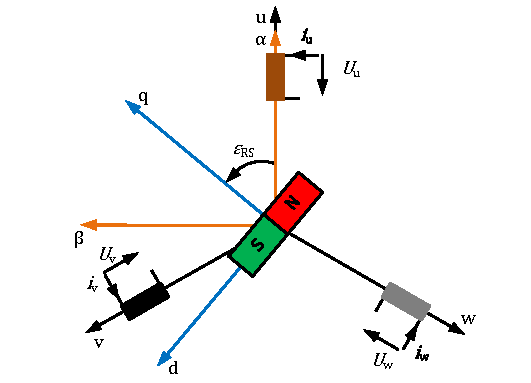
\includegraphics[width=\columnwidth]{img/synchron-grundlage}
\caption{Graphische Veranschaulichung der verschiedenen Koordinatensysteme, ständerfest $(\alpha, \beta)$ und rotorfest $(d, q)$.}
\label{fig:synchron-grundlage}
\end{figure}

\shortpage

Durch Trennung von Real- und Imaginärteil ergibt sich die üblicherweise verwendete Spannungsleichung im rotorfesten System zu \autocites{schroder2001}{nuss2010}:

\begin{align}
u_\x{d} &= R_\x{1} i_\x{d} + \frac{\x{d}}{\x{d}t}\Psi_\x{d} - \omega_{\x{el}} \Psi_\x{q} \label{eqn:ud} \\ 
u_\x{q} &= R_\x{1} i_\x{q} + \frac{\x{d}}{\x{d}t}\Psi_\x{q} + \omega_{\x{el}} \Psi_\x{d} \label{eqn:uq}
\end{align}

Allgemein lässt sich das daraus resultierende innere Drehmoment als

\begin{align}
M_\x{i} = \frac{3}{2} (\underline{\Psi}^{\x{d,q}} \times \underline{i}^{\x{d,q}}) \label{drehmoment}
\end{align}

beschreiben.
Dabei wird vorausgesetzt, dass die Ständerwicklung symmetrisch und dreiphasig ist, der Strombelag sinusförmig über dem Umfang verteilt ist und kein Nullsystem vorliegt \autocite{schroder2001}.
Das innere Drehmoment $M_\x{i}$ für eine Maschine mit $p$ Polpaaren kann nach der Berechnung des Vektorproduktes als

\begin{align}
M_\x{i} = \frac{3p}{2}(\Psi_\x{d} i_\x{q} - \Psi_\x{q} i_\x{d})
\end{align}

geschrieben werden.
Um das System vollständig zu beschreiben fehlt noch die Bewegungsgleichung:

\begin{align}
M_\x{i} - M_\x{Last} = J \frac{\x{d}}{\x{d}t} \omega_{\x{mech}} \label{bewegungsgleichung}
\end{align}

Bei diesem Modell sind alle Parameter konstant~--~die Ableitungen der Flussverkettungen, die in Gl.~(\ref{eqn:ud}) und Gl.~(\ref{eqn:uq}) verwendet werden, sind einfach zu bestimmen.
Aufgrund von Sättigungseffekten des Eisens sind insb.\ bei hochausgenutzten Maschinen die Induktivitäten der Synchronmaschine nicht mehr konstant, sondern vom Motorstrom abhängig.

\subsection{Linearisierte Gleichungen}\label{sec:lin-gleichungen}

Bei dem linearisierten Modell sind definitionsgemäß keine Sättigungserscheinungen vorhanden \autocite{mullerII2008}.
Alle elektrischen Parameter der permanentmagneterregten Synchronmaschine und damit auch die Induktivitäten sind damit konstant.
Aus dieser Annahme folgt, dass sich die rotofesten $d, q-$Komponenten zu

\begin{align}
\Psi_\x{d} &= \Psi_\x{pm} + L_\x{d} i_\x{d} \label{eqn:psid}\\
\Psi_\x{q} &= L_\x{q} i_\x{q} \label{eqn:psiq}
\end{align}

ergeben \autocite{schroder2001}.

Die in $d-$Achse ausgerichteten Permanentmagnete rufen eine als konstant angenommene Flussverkettung $\Psi_\x{pm}$ hervor.
Daraus ergeben sich in Gl.~(\ref{eqn:ud}), Gl.~(\ref{eqn:uq}) und Gl.~(\ref{drehmoment}) eingesetzt die Grundgleichungen des linearen Maschinenmodells zu:

\begin{align}
u_\x{d} &= R_\x{1} i_\x{d} + L_\x{d} \frac{\x{d}i_\x{d}}{\x{d}t} - \omega_\x{el}L_\x{q} i_\x{q}  \label{uq-allg} \\ 
u_\x{q} &= R_\x{1} i_\x{q} + L_\x{q} \frac{\x{d}i_\x{q}}{\x{d}t} + \omega_\x{el}L_\x{d} i_\x{d} + \omega_\x{el}\Psi_\x{pm} \label{ud-allg} \\ 
M_\x{i} &= \frac{3p}{2}(\Psi_\x{pm} i_\x{q} + (L_\x{d} - L_\x{q})i_\x{d} i_\x{q})
\end{align}

Die Spannungsgleichungen lassen sich gemäß Abb.~\ref{fig:spannungsgleichungen} graphisch darstellen.

\begin{figure}[!h]
\centering
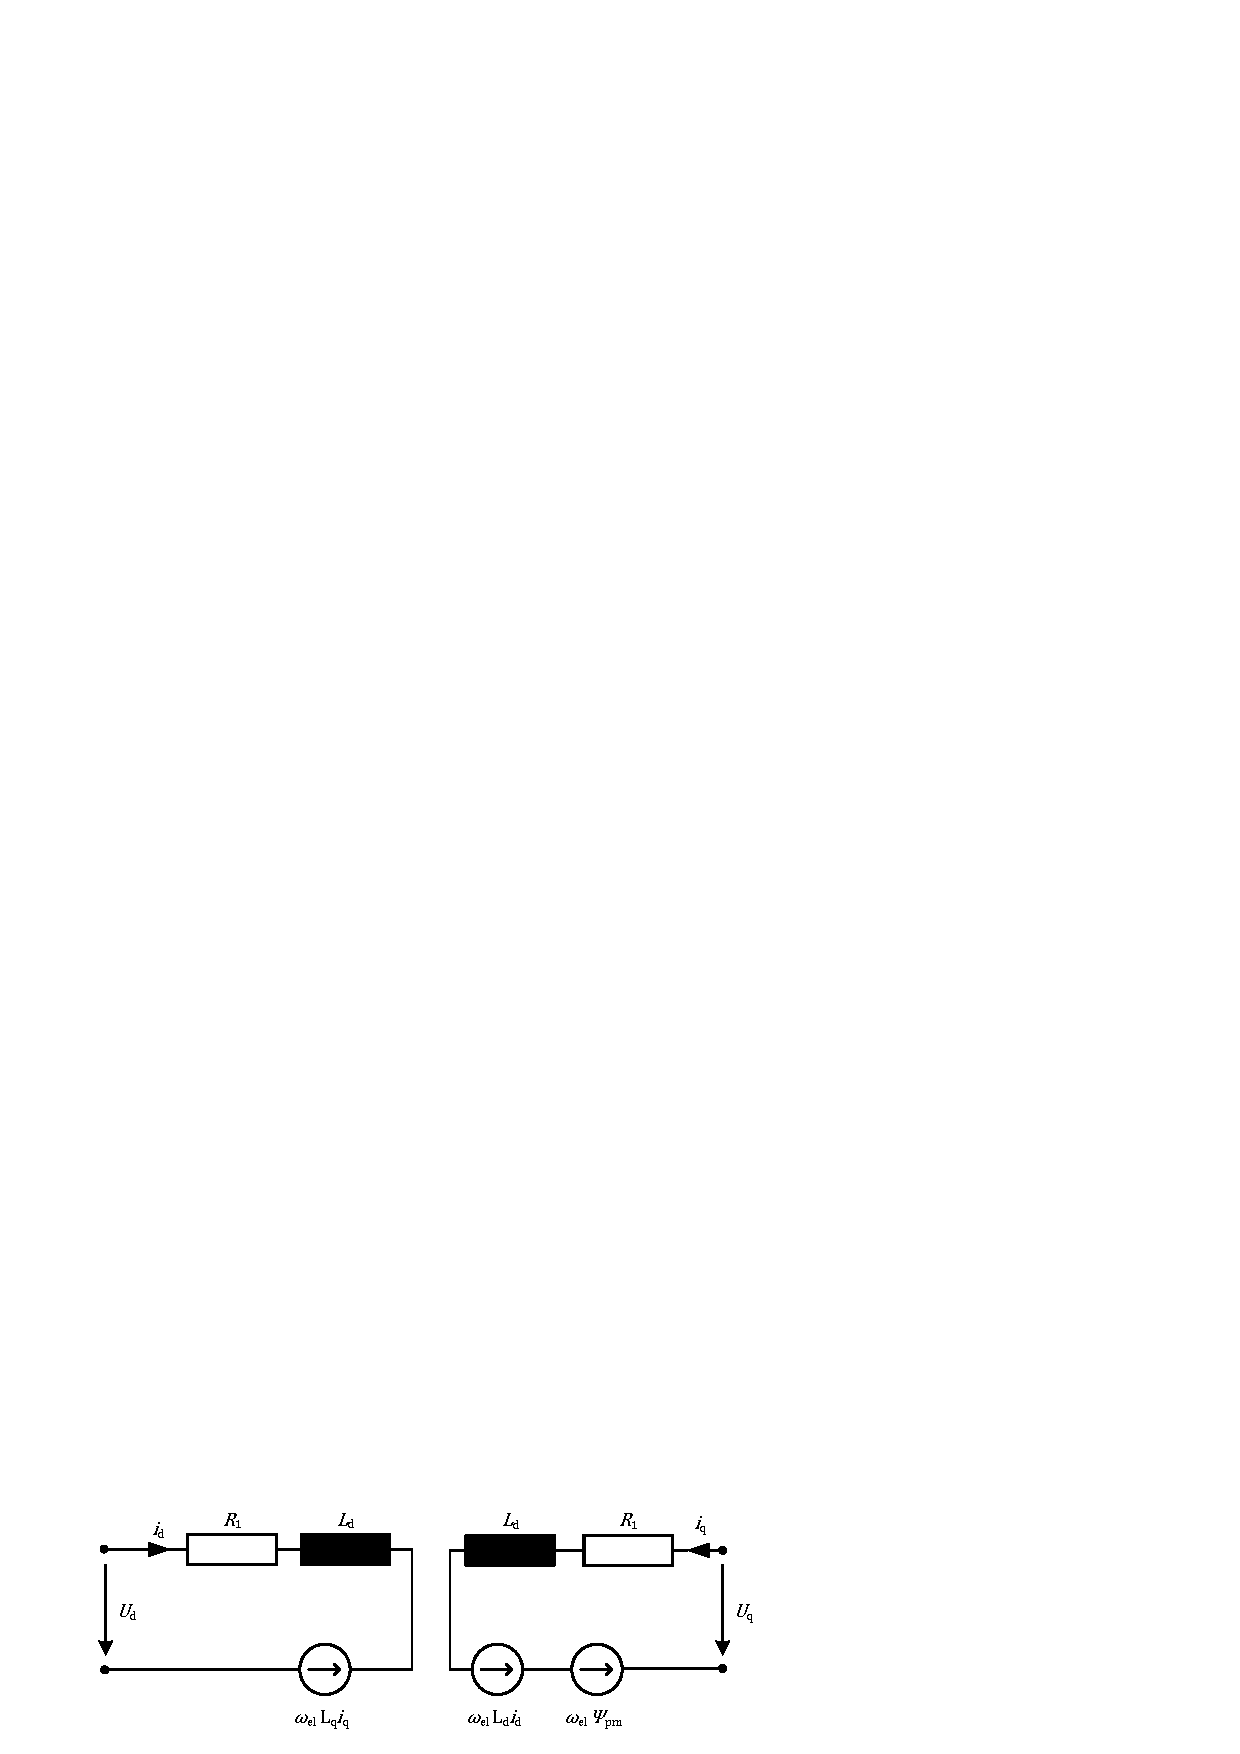
\includegraphics[width=\columnwidth]{img/spannungsgleichungen}
\caption{Graphische Darstellung der Gleichungen Gl.~(\ref{uq-allg}) und Gl.~(\ref{ud-allg}).}
\label{fig:spannungsgleichungen}
\end{figure}

Erkennbar ist, dass in der Abb.~\ref{fig:spannungsgleichungen} die Spannungsquellen $\omega_\x{el} L_\x{q} i_\x{q}$ und $\omega_\x{el} L_\x{d} i_\x{d}$ miteinander verkoppelt sind.
Löst man oben stehende Gl.~(\ref{uq-allg}),(\ref{ud-allg}) mit der Bewegungsgleichung Gl.~(\ref{bewegungsgleichung}), so ergibt sich folgendes Gleichungssystem:

\begin{align}
\frac{\x{d}i_\x{d}}{\x{d}t} &= -\frac{R_\x{1}}{L_\x{d}}i_\x{d}+\omega_\x{el}\frac{L_\x{q}}{L_\x{d}}i_\x{q}+\frac{1}{L_\x{d}}u_\x{d} \\
\frac{\x{d}i_\x{q}}{\x{d}t} &= -\omega_\x{el}\frac{L_\x{d}}{L_\x{q}}i_\x{d} - \frac{R_\x{1}}{L_\x{q}}i_\x{q} + \frac{1}{L_\x{q}}u_\x{q} - \frac{\omega_\x{el}}{L_\x{q}}\Psi_\x{pm} \\
\frac{\x{d}\omega_\x{el}}{\x{d}t} &= \frac{3p^2}{2J}(L_\x{d} - L_\x{q})i_\x{q} i_\x{d} + \frac{3p^2}{2J} \Psi_\x{pm} i_\x{q} - \frac{p}{J} M_\x{Last}
\end{align}

\subsection{Allgemeine Maschinen Gleichungen}\label{sec:allg-gleichungen}

Bei jeder permanentmagneterregten Synchronmaschine ändern sich die Induktivitäten in Abhängigkeit von der Last.
In erster Linie sind dafür die Sättigungseffekte, aber auch die Kreuzkopplung verantwortlich.
Die Kreuzkopplung entsteht durch die gegenseitige Beeinflussung der verkoppelten Induktivitäten der $d-$ und $q-$Achsen des rotorfesten Systems.
Da z. B. in der realen Maschine beide Flüsse in dem gleichen Ständerblech verlaufen, ist es nachvollziehbar, dass ein $i_\x{d}-$Strom eine Vorsättigung des Blechs verursacht und in der Folge bei einem zusätzlich eingeprägten $i_\x{q}-$Strom die Sättigung des Blechs früher eintritt.
Bei der Verwendung der linearen Gleichungen (s.~h.~Abschn.~\ref{fig:spannungsgleichungen}) war die Definition des Flussverkettung (s.~h.~Gl.~(\ref{eqn:psid}) und Gl.~(\ref{eqn:psiq})).
Bei Berücksichtigung der Eisenverluste sind die Induktivitäten nicht mehr konstant, sondern ändern sich in abhängigkeit der Last.
Aus diesen Betrachtungen folgen die neuen Gleichungen für $\Psi_\x{d}$ und $\Psi_\x{q}$:

\begin{align}
\Psi_\x{d} &= \Psi_\x{pm} + L_\x{dd}^{\xi}(i_\x{d})\cdot i_\x{d} + L_\x{dq}^{\xi}(i_\x{d} ,i_\x{q})\cdot i_\x{q} \\
\Psi_\x{q} &= L_\x{qq}^{\xi}(i_\x{q})\cdot i_\x{q} + L_\x{qd}^{\xi}(i_\x{d} ,i_\x{q})\cdot i_\x{d}
\end{align}

Die Selbstinduktivitäten $L_\x{dd}^{\xi}$ und $L_\x{qq}^{\xi}$ beschreiben, die Induktivitäten, die allein durch den \emph{eigenen} Strom hervorgerufen wurden.
Das hochgestellte $\xi$ soll die Berücksichtigung der Eisenverluste darstellen.
Die Gegeninduktivitäten $L_\x{dq}^{\xi}$ und $L_\x{qd}^{\xi}$ beschreiben den Anteil, den der jeweils andere Strom hervorruft.
Es ist möglich, Induktivitäten gemäß \textcite{Kellner2012}

\begin{align}
	L_\x{d}^{(i_\x{d},i_\x{q})}	&=	L_\x{dd}^{\xi}(i_\x{d})+L_\x{dq}^{\xi}(i_\x{d},i_\x{q})\cdot\frac{i_\x{q}}{i_\x{d}} \label{eqn:induktiv-neu-1} \\
	L_\x{q}^{(i_\x{d},i_\x{q})}	&=	L_\x{qq}^{\xi}(i_\x{q})+L_\x{qd}^{\xi}(i_\x{d},i_\x{q})\cdot\frac{i_\x{d}}{i_\x{q}} \label{eqn:induktiv-neu-2}
\end{align}

zu definieren.
Um die Abhängigkeit der Induktivitäten von den Strömen beschreiben zu können und eine möglichst kurze Darstellung zu erreichen, wir die Abhängigkeit im Folgenden durch den Exponenten dargestellt.
Analog zu den oben beschriebenen Gleichungen (s.~h.~Gl.~(\ref{eqn:psid}) und Gl.~(\ref{eqn:psiq})) lassen sich die Flüsse umschreiben zu:

\begin{align}
\Psi_\x{d}^{(i_\x{d},i_\x{q})} &= \Psi_\x{pm}^{(i_\x{d},i_\x{q})} + L_\x{d}^{(i_\x{d},i_\x{q})}\cdot i_\x{d} \\
\Psi_\x{q}^{(i_\x{d},i_\x{q})} &= L_\x{q}^{(i_\x{d},i_\x{q})}\cdot i_\x{q}
\end{align}

Die obige Definition ist sinnvoll; in Folge ergeben sich nicht nur kürzere mathematische Ausdrücke, sondern ist es auch für die praktische Anwendung nicht ersichtlich, welchen Mehrwert die Trennung in Selbst- und Gegeninduktivität hat.
Ein weiterer Vorteil ist es, dass die erweiterten Gleichungen in die linearisierte Form überführbar sind.
Durch einige Umformungen ergibt sich nach \textcite{Kellner2012} folgendes Gleichungssystem:

\begin{align}
\left( \begin{array}{c} u_\x{d} \\ u_\x{q} \end{array} \right) &= \left( \begin{array}{cc} R_\x{1} & -\omega_\x{el}L_\x{q}^{(i_\x{d},i_\x{q})} \\ \omega_\x{el}L_\x{d}^{(i_\x{d},i_\x{q})} & R_\x{1} \end{array} \right) \left(\begin{array}{c} i_\x{d} \\ i_\x{q} \end{array}\right) \label{eqn:allg-spannungsgleichung} \\ 
 &\ldots + \underbrace{\left( \begin{array}{cc} L_\x{dd}^{(i_\x{d},i_\x{q})} & L_\x{dq}^{(i_\x{d},i_\x{q})} \\ L_\x{qd}^{(i_\x{d},i_\x{q})} & L_\x{qq}^{(i_\x{d},i_\x{q})} \end{array}\right)}_{\text{differentielle Induktivitäten}} \left(\begin{array}{c} i_\x{d} \\ i_\x{q} \end{array} \right) \nonumber \\ 
& \ldots + \left( \begin{array}{c} \frac{\x{\partial}}{\x{\partial }t} \Psi_\x{pm}^{(i_\x{q})} \\ \omega_\x{el} \Psi_\x{pm}^{(i_\x{q})} \nonumber \end{array}  \right) \nonumber
\end{align}

Um zur Drehmomentgleichung zu gelangen, lassen sich ausgehend von der allgemeinen Darstellung die Flussverkettungen ersetzen:

\begin{align}
M_\x{i} = \frac{3p}{2}\left( \Psi_\x{pm}^{(i_\x{q})}\cdot i_\x{q} + (L_\x{d}^{(i_\x{d},i_\x{q})}-L_\x{q}^{(i_\x{d},i_\x{q})})i_\x{d} i_\x{q}\right)
\end{align}

Wird nun noch die mechanische Bewegungsgleichung eingefügt ergibt sich:

\begin{small}
\begin{align}
\frac{J}{p}\frac{\x{d}\omega_\x{el}}{\x{d}t} &= \frac{3p}{2}(\Psi^{(i_\x{q})}_\x{pm}i_\x{q} + (L^{(i_\x{d},i_\x{q})}_\x{d}-L^{(i_\x{d},i_\x{q})}_\x{q})i_\x{d} i_\x{q}) - M_\x{Last} \label{eqn:allg-drehmoment}
\end{align}
\end{small}

Aus diesen drei Gleichungen lassen sich allgemeine mathematische Modelle zur Simulation einer Synchronmaschine erstellen. 
Für Grundlagen im Bereich der elektrischen Maschinen wird auf einschlägige Literatur verwiesen \autocites{mullerII2008}{mullerI2005}{fischer2009}{schroder2001}.

\begin{figure}[!h]
\centering
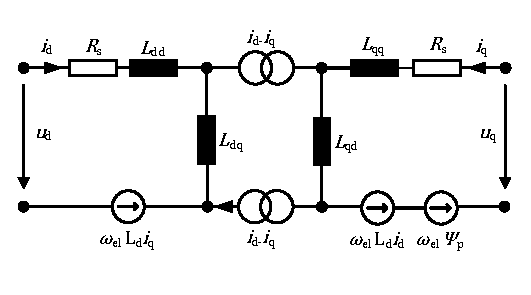
\includegraphics[width=\columnwidth]{img/allg-spannungsgleichung}
\caption{Graphische Darstellung der Gleichungen (Gl.~\ref{eqn:allg-spannungsgleichung}) und Gl.~(\ref{eqn:allg-drehmoment}).}
\label{fig:allg-spannungsgleichung}
\end{figure}

Im Unterschied zu den linearisierten Spannungsgleichungen (s.~h.~Gl.~(\ref{uq-allg}) und Gl.~(\ref{ud-allg})), sind die beiden Spannungsgleichungen (s.~h.~Gl.~(\ref{eqn:allg-spannungsgleichung})) zusätzlich durch die Anteile der differentiellen Induktivitäten $L_\x{dq}$ und $L_\x{qd}$ verkoppelt.
Wie in der Abb.~\ref{fig:allg-spannungsgleichung} zu sehen ist, werden zwei Stromquellen integriert.
Sind die beiden Induktivitäten $L_\x{dq}$ und $L_\x{qd}$ gleich null, so ergibt sich ein ähnliches Ersatzschaltbild wie in Abb.~\ref{fig:spannungsgleichungen}.
Lediglich die Selbstinduktivitäten $L_\x{dd}$ und $L_\x{qq}$ sind durch die Induktivitäten $L_\x{d}$ bzw. $L_\x{q}$ ersetzt.

\section{Ansätze zur Identifikation}\label{sec:identifikation}
\subsection{Ansätze zur Berechnung der Rotorposition}\label{sec:rotorposition}

Um die Parameter einer permanentmagneterregten Synchronmaschine identifizieren zu können, ist es notwendig, die korrekte Lage des Rotors zu ermitteln \autocites{underwood_online_2010}{rahman_identification_2005}{piippo_adaptation_2009}.
Mit Hilfe eines Resolvers, Inkrementalgebers oder eines Absolutwertgeber wird die Rotorlage ermittelt.
Die Implementierung solcher Messeinrichtungen ist mit Kosten und Wartungsaufwand verbunden.
An dieser Stelle soll deshalb auf eine geberlose Regelung eingegangen werden.
Wie die Bezeichnung schon nahelegt, wird bei der geberlosen Regelung auf den Drehgeber verzichtet.
Bei einer geberlosen Regelung werden i.\ d.\ R.\ aus den drei Phasenströmen der Läuferlagewinkel $\epsilon_\x{RS}$ berechnet, wobei von den drei Phasenströmen nur zwei gemessen werden und der dritte aus ihnen berechnet wird \autocite{ternesfeldkamp}.
Es gibt unzählige Veröffentlichungen in diesem Forschungsbereich; dabei werden auch unterschiedliche Verfahren zur Realisierung dargestellt.
Ausgehend vom Maschinenmodell der permanentmagneterregten Synchronmaschine (s.~h.~Abschn.~\ref{sec:math-pmsm}), wird an dieser Stelle eine Klassifizierung der Methoden in die folgenden Klassen vorgenommen:

\begin{itemize}
	\item Methoden basierend auf dem Grundwellenmodell der Maschine
	\item Methoden basierend auf den Anisotropien der Maschine
\end{itemize}

Die Methoden \enquote{basierend auf dem Grundwellenmodell} nutzen die im Grundwellenmodell betrachteten induzierten Spannungen zur indirekten Bestimmung der Rotorposition \autocite{Perassi2006}.
Dabei werden die Grundschwingungsgrößen der Ständerspannung $U_\x{1}$ und der Ständerstroms $I_\x{1}$ als Eingangssignale des Modells betrachtet.
Da eine Strommessung bei geregelten Antrieben mit Frequenzumrichter i.\ d.\ R.\ ohnehin vorhanden ist, wird keine zusätzliche Messeineinrichtung benötigt.
Die Ausgangsspannung wird dann über die Pulsweitenmodulation gemessen, dabei muss die Nichtlinearität des Wechselrichters betrachtet werden.
Bei der Bestimmung der Rotorposition im Stillstand kann dieses Verfahren keine Ergebnisse liefern.
Ebenso ist es schwierig bei niedrigen Drehzahlen die Ausgangsspannung am Wechselrichter zu messen, da die induzierte Spannung zu gering ist.
Dieses Verfahren ist nur für eine Beschränkung des Drehzahlbereichs anwendbar.
Andere Verfahren zur Rotorbestimmung sind u.\ a.\ sehr theoretische Verfahren, wie z.\ B.\ Zustandsbeobachter oder Kalman-Filter.
Diese Verfahren sind nach aktuellen Stand nicht industrietauglich \autocite{Kellner2012}.
Im Weiteren wird zwischen zwei Verfahren unterschieden:

\begin{itemize}
\item Passive Verfahren, bei denen die Bestimmung erfolgt, ohne die für die feldorientierte Regelung normale Pulsweitenmodulation zu beeinflussen
\item Aktive Verfahren, bei denen Umrichterzustände oder Testsignale eingefügt werden, um die Effekte der induzierten Spannung zu verdeutlichen
\end{itemize}

Methoden basierend auf den Anisotropien der Maschine sollen im Weiteren nicht behandelt werden, hierfür wird auf einschlägige Literatur verwiesen \autocites{Perassi2006}{kiel2005}.
In \textcite{kiel2005} werden auch die Effekte, die zur Änderung der Induktivität mit der Rotorlage führen erörtert.
Im Rahmen einer geberlosen Regelung ist es enorm wichtig, dass die absoluten und differentiellen Induktivitäten bekannt sind (s.~h.~Abschn.~\ref{sec:induktiv}).

\subsection{Ansätze zur Identifikation der Induktivitäten}\label{sec:induktiv}

Innerhalb der feldorientierten Regelung werden die absoluten Induktivitäten z. B. für die Berechnung des Spannungssollwertmodells, der Vorsteuerung, benötigt.
Auch bei den Ansätzen der Ständeridentifikation werden die Induktivitäten benötigt (s.~h.~Abschn.~\ref{sec:stator-ident}).
Da für die praktische Anwendung vor allem die Parameter in rotorfesten Koordinaten von Belang sind, beschränkt sich auch die Darstellung der Induktivitäten in diesem Abschnitt auf das rotorfeste Koordinatensystem.
Die Identifikation der Induktivitäten wird ausschließlich offline durchgeführt.

\begin{quote}
\enquote{Zum einen ändern sich die Induktivitäten im Wesentlichen nur abhängig von den Strömen $i_\x{d}$ und $i_\x{q}$, kaum aufgrund von anderen äußeren Umgebungseinflüssen beziehungsweise Prüfstandsparametern, wie zum Beispiel Temperatur oder Drehzahl des Systems \autocite[S.~79]{Kellner2012}.}
\end{quote}

Eine Onlinemessung ist nicht erforderlich~--~im Gegensatz zur Ständerwiderstandsidentifikation.
Onlinemessverfahren sind entweder gar keine richtigen \enquote{online}-Verfahren oder haben eine zweifelhafte Stabilität und Genauigkeit \autocite{underwood_online_2010}.
Ein echte Onlineidentifikation der Induktivitätsverläufe ist in \autocite{underwood_online_2010} beschrieben.
Zu dem Vorteilen schreibt \textcite{underwood_online_2010}, dass es sinnvoll ist die Parameter online zu bestimmen:

\begin{quote}
\enquote{Using an online parameter estimation algorithm allows the controller to have precise parameter estimates even when these are subject to perturbation, regardless of its origin. Consequently, phenomena like temperature effects and cross-saturation can be accounted for through their effect on the machine parameters, which is difficult with an offline method \autocite[S.~1]{underwood_online_2010}.}
\end{quote}

Allerdings dauert das Nachführen der identifizierten Induktivität zu lange für die schnell ablaufenden transienten Vorgänge.
Gerade bei sprunghaften Änderungen des Stromes müssen sich die Induktivitäten im Modell schnell ändern, ansonst kann man auf variable Induktivitäten verzichten \autocite{Kellner2012}.
Das in \autocite{underwood_online_2010} beschriebene Onlineidentifikationsverfahren eignet sich nur für quasistationäre Zustände in Antriebssystemen.

Bei den Darstellungen der Induktivitäten unterscheidet man zwischen \emph{absoluten Induktivitäten, Sekanteninduktivitäten} $L = \frac{\Psi}{i}$ und \emph{differentiellen Induktivitäten} $L = \frac{\x{d}\Psi}{\x{d}i}$, welche die Steigung der Tangente angibt.

\begin{figure}[!h]
\centering
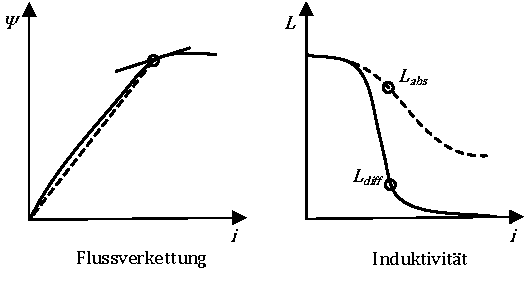
\includegraphics[width=\columnwidth]{img/induktiv}
\caption{Prinzipielle Darstellung der Beziehung zwischen absoluter und differentieller Induktivität in Anlehnung an \textcite[S.~2]{kellner_general_2011}. Rechts: Durchgezogenen Linie stellt den Verlauf des Flusses dar, die Tangente in dem Arbeitspunkt soll die differentielle Induktivität darstellen. Die gestrichelte Linie stellte die Sekante der absoluten Induktivität dar. Links: Prinzipieller Verlauf des absoluten und differentiellen Induktivität, ein beispielhafter Arbeitspunkt ist eingezeichnet.}
\label{fig:induktiv}
\end{figure}

Für die Identifikation der absoluten Induktivität in der Praxis lässt sich die Vorgehensweise wie folgt schildern:

\begin{itemize}
\item Die Regelung der zu prüfenden Maschine muss so aufgebaut sein, dass jede mögliche Kombination aus $i_\x{d}-$ und $i_\x{q}-$Strömen eingestellt werden kann. Die Lastmaschine muss einen kostanten Drehzahlsollwert realisieren können \autocite{Kellner2012}.
\item Es muss eine konstante Drehzahl eingestellt werden, bei niedrigen Drehzahl ist die induzierte Spannung so gering, dass diese durch die Umrichterlinearisierungsfehler die Messergebnisse verfälschen kann \autocite{Perassi2006}. Bei zu hohen Drehzahlen wirken sich drehzahlabhängige Fehler, wie z. B. die Eisenverluste, negativ auf die Messergebnisse aus.
\item Über den gesamten zu messenden Bereich werden automatisierte Betriebspunkte eingestellt. Sobald sich ein stationärer Zustand eingestellt hat, werden alle für die Identifikation der absoluten Induktivität benötigten Messwerte gespeichert.
\item Die gemessenen Werte müssen ausgewertet und die Induktivität anhand des Referenzmodells berechnet werden.
\end{itemize}

Bei diesem Verfahren wird davon ausgegangen, dass die Permanentmagnetflussverkettung $\Psi_\x{pm}$ nicht bekannt ist, so wird:

\begin{quote}
\enquote{Um $\Psi_\x{p}$ zu gewinnen [\ldots], wird $\Psi_\x{d}$ im Zähler der Induktivitätsgleichung zeilenweise variiert, bis jeweils der Offset für eine Zeile verschwunden
ist. Die Differenz zwischen variierter Flussverkettung und $\Psi_\x{d}$ entspricht in diesem Fall der Permanentmagnetflussverkettung $\Psi_\x{pm}$ \autocite[S.~109]{Kellner2012}.}
\end{quote}

Dabei ist die Gleichung für die absolute Induktivität definiert als (s.~h.~Abb.~\ref{fig:induktiv}, beispielhafte Arbeitspunkte sind eingezeichnet):

\begin{align}
L_\x{d} = \frac{\Psi_\x{d}}{i_\x{d}}
\end{align}

Für die Berechnung der Induktivität in $q-$Richtung ist die Vorgehensweise die gleiche, allerdings ist $L_\x{q}$ im Vergleich zu $L_\x{d}$ weitgehend offsetfrei.
Im Idealfall gilt für $L_\x{q}$:

\begin{align}
L_\x{q} = \frac{\Psi_\x{q}}{i_\x{q}}
\end{align}

%\begin{figure}[!h]
%\centering
%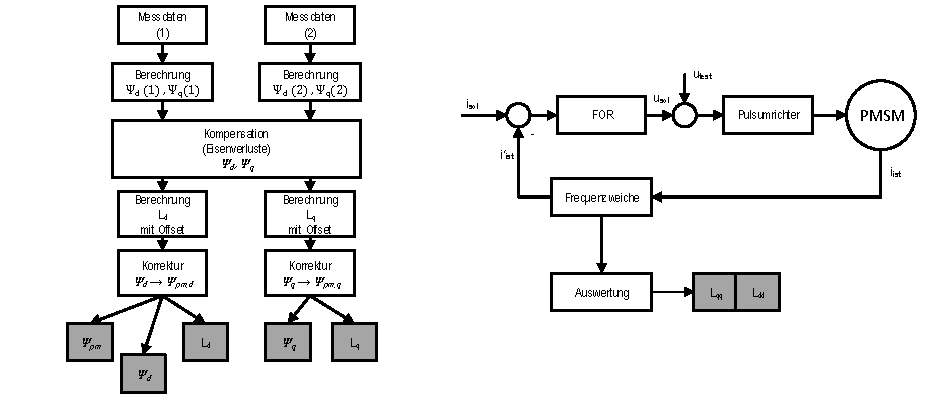
\includegraphics[width=\textwidth]{img/induktiv-kellner}
%\caption{Verfahren zur Bestimmung der absoluten bzw. differentiellen Induktivität in Anlehnung an \textcite{Kellner2012}. Links: Verarbeitung der Messdaten zur Bestimmung der absoluten Induktivitäten. Rechts: Vereinfachte Struktur der Testsignalerzeugung und Auswertung bei Verwendung von Spannungstestsignalen.}
%\label{fig:induktiv-absolut-diff}
%\end{figure}

%Bei den differentiellen Induktivitäten handelt es sich um Induktivitäten die mit der Stromänderung zusammenhängen, also während dynamischer Vorgänge.
%Die differentiellen Induktivitäten sind in den allgemeinen Spannungsgleichungen für permanentmagneterregte Synchronmaschinen enthalten.

%\emph{Testsignale für niedrige Drehzahlen:}

%\emph{EMK-Verfahren für hohe Drehzahlen:} Im Gegensatz zu dem beschriebenen Testsignalverfahren, welches aktiv in das Antriebssystem eingreift, ergeben sich bei hohen %Drehzahlen genügend passive Verfahren zur Bestimmung der Rotorlage.

%\begin{quote}
%\enquote{[\ldots] Eine Drehzahl ist immer dann für das EMK-Verfahren ausreichend, wenn die angelegten Spannungen so groß sind, dass der Rauschanteil auf den gemessenen oder %berechneten Spannungen vernachlässigbar klein ist. [\ldots] \autocite[S.~48]{Kellner2012}}
%\end{quote}

%Basis für solche EMK-Modelle sind die in Abschn.~\ref{sec:lin-gleichungen} beschriebenen Gleichungen.
%Dabei wird von einem linearen Verhalten im Betriebsbereich ausgegangen \autocite{piippo_adaptation_2009}.

\subsection{Ansätze zur Identifikation des Ständerwiderstands}\label{sec:stator-ident}

Der Ständerwiderstand $R_\x{1}$ ist eine wichtige Kenngröße für den Betrieb elektrischer Maschinen.
Bei dem modellbasierten EMK-Verfahren für kleine Drehzahlen, z. B. \autocite{genduso}, ist es notwendig eine möglichst genaue Identifikation des Ständerwiderstandes zu bekommen.
Im Folgenden werden einige Beispiele zur Identifikation des Ständerwiderstandes anhand aktueller Veröffentlichungen dargestellt.

Die Auswertung der $u_\x{d}-$ oder $u_\x{q}-$Spannungsgleichung: Zur Auswertung der $u_\x{d}$-Gleichung ist ein $d-$Strom ungleich null Voraussetzung, was die praktische Anwendung stark einschränkt \autocite{Kellner2012}.
Die Auswertung der $u_\x{q}-$Gleichung liefert immer dann gute Ergebnisse, wenn gleichzeitig hohe $i_\x{d}-$Ströme und kleine Drehzahlen vorhanden sind.
Für die Antriebe, die aus dem Stand anfahren, ist dies kein Nachteil.
%Es gibt auf dem Gebiet \enquote{Verfahren zur Identifikation der Parameter von permanenterregten Synchronmaschinen} viele Veröffentlichungen.
Einige Ansätze verwenden den MRAC-Algorithmus (model-reference adaptive control) zur Identifikation des Ständerwiderstandes \autocite{slotine_applied_1991}.
Der prinzipielle Aufbau ist in Abb.~\ref{fig:synchron-grundlage} gezeigt.

\begin{figure}[h!]
\centering
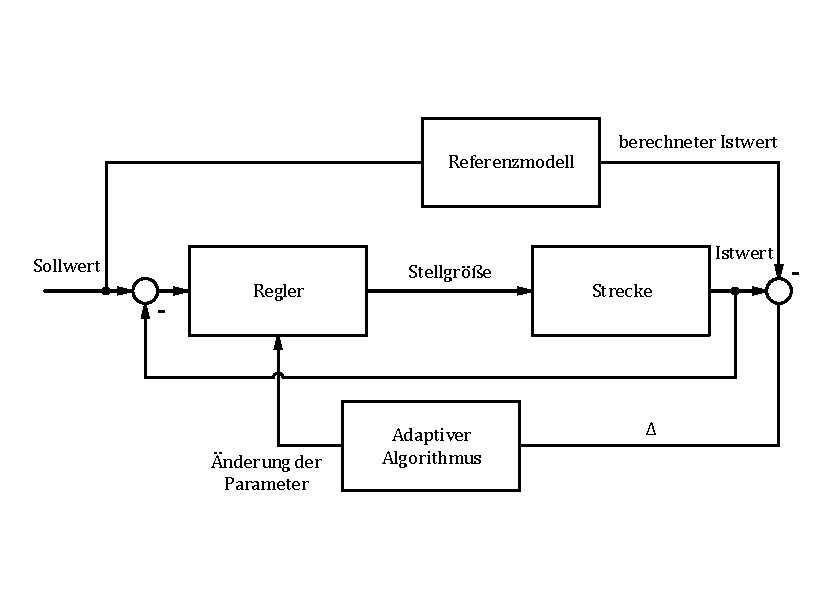
\includegraphics[width=\columnwidth]{img/mrac}
\caption{Prinzipielle Darstellung eines \texttt{MRAC}-Algorithmus in Anlehnung an \textcite{slotine_applied_1991}.}
\label{fig:mrac}
\end{figure}

Wenn bekannt ist, welchen Verlauf die Ausgangsgröße der Strecke bei einer bestimmten Eingangsgröße haben soll, dann kann diese mathematische Beziehung in einem Referenzmodell hinterlegt werden.
Der Algorithmus ist in \autocite{slotine_applied_1991} genauer beschrieben (s.~h.~Abb.~\ref{fig:mrac}).
Bei der Parameteridentifikation kann das mathematische Referenzmodell die Gleichungen der permanentmagneterregten Synchronmaschine beschreiben, der Regler passt über den Ständerwiderstand die unbekannte Strecke an, bis sie den idealen Maschinengleichungen entsprechen.
Sind die Parameter der Maschine nicht genau bekannt, dann ist es nicht möglich ein genaues Referenzmodell zu erstellen.
Eine andere Möglichkeit zur Identifikation des Ständerwiderstandes ist die Einprägung von Testsignalen in $d-$ und $q-$Richtung.
Die Auswertung der eingeprägten Signale liefert dann die Spannungs- bzw.\ Stromantwort.
In \autocite{wilson2005} wird eine Methode beschrieben, mit der durch Injektion eines Stromraumzeigers der Widerstand und damit auch die Temperatur der Ständerwicklung bestimmt wird.
Das Verfahren zur Bestimmung dieser Maschinenparameter wurde bisher nur simuliert und nicht verifiziert.
Der entscheidende Nachteil dieses Prinzips ist, dass auch die Ständeridentifikation nur funktioniert, wenn das hochfrequente Testsignal vorhanden ist, also nur bei geringen Drehzahlen.
Patentierte Identifikationsverfahren auf dem Gebiet sind in \autocites{schutzrecht1}{schutzrecht2} ausführlich beschrieben.
Weitere Ansätze zur Identifikation des Ständerwiderstandes sind in \textcite{Kellner2012} beschrieben.
Diese Verfahren benötigen keine Testsignale und werten die bekannten Spannungsgleichungen in $d-$ oder in $q-$Richtung in rotorfesten Koordinaten aus.
Diese Möglichkeit gilt nicht für alle Betriebsbereiche. 
Aus diesem Grund wird ein weiteres Verfahren eingeführt, welches robust und resourcenschonender ist.
Durch die Injektion eines niederfrequenten $i_\x{d}$-Strom-Testsignales kann die $u_\x{d}4$-Spannungsgleichung ausgewertet werden.

\begin{figure}[!h]
\centering
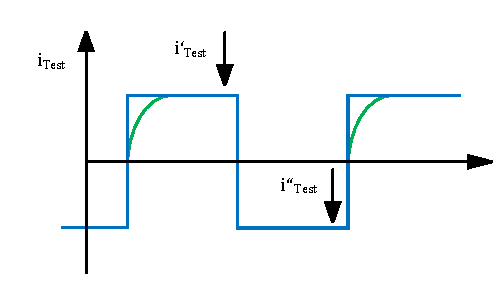
\includegraphics[width=2.5in]{img/test-strom}
\caption{Prinzipieller Teststromverlauf, Blau: Idealer Stromverlauf. Grün: Realer Stromverlauf.}
\label{fig:test-strom}
\end{figure}

Der gesamte Identifikationsprozess läuft innerhalb des rotorfesten $d, q-$Koordinatensystems ab.
Prinzipiell können sowohl die $u_\x{d}$-Spannungsgleichung, als auch die $u_\x{q}$-Spannungsgleichung verwendet werden.

\begin{quote}
\enquote{Die $u_\x{q}-$Gleichung scheidet jedoch aus: Der benötigte alternierende $i_\x{q}$-Teststrom würde ein unerwünschtes Pendelmoment erzeugen.}\autocite[S.~148]{Kellner2012}
\end{quote}

Der Einfluss in $d-$Richtung auf das abgegebene Drehmoment ist wesentlich geringer.
Damit kann die Gleichung für den identifizierten Ständerwiderstand nach \textcite{Kellner2012} geschrieben werden als:

\begin{small}
\begin{align}
R_\x{1,ident} = \frac{u_\x{d}'' - u_\x{d}' + \omega_\x{el}'' L_\x{q}^{(i_\x{d}'',i_\x{q}'')}\cdot i_\x{q}'' - \omega'_\x{el}L_\x{q}^{(i_\x{d}',i_\x{q}')}i_\x{q}'}{i_\x{d}''-i_\x{d}'}
\end{align}
\end{small}

Wenn die Induktivitäten bekannt sind, kann der Ständerwiderstand berechnet werden.
Unter Bezugnahme der Ständertemperatur ergibt sich dann für den identifizierten Ständerwiderstand nach \autocite{Kellner2012}:

\begin{align}
R_\x{1} = R_\x{1,20^{\circ}\x{C}}\cdot \left[ 1 + \alpha_\x{Cu}(\vartheta_\x{1} - 20^{\circ}\x{C})\right]
\end{align}

$R_\x{1,20^{\circ}\x{C}}$ beschreibt den gemessenen Ständerwiderstand bei einer Umgebungstemperatur von $20^{\circ}\x{C}$, $\vartheta_\x{1}$ die aktuelle Ständertemperatur und $\alpha_\x{Cu}$ den Temperaturkoeffizient von Kupfer.


\subsection{Identifikation der Flussverkettung}\label{sec:ident-fluss}

Für die Identifikation der Flussverkettung $\Psi_\x{pm}$ kann das gleiche Testsignale in $d-$Richtung verwendet werden, wie bei der Identifikation des Ständerwiderstandes.
Bei der Identifikation des Flusses werden nur stationäre Zustände betrachtet, daher können die Ableitungen der Ströme weggelassen werden, da sie im Mittel ohnehin null ergeben \autocite{Kellner2012}.
Für die Identifikation des Flusses wird die $u_\x{q}-$Gleichung (s.~h.~Gl.~(\ref{uq-allg})) verwendet.
Da der Teststrom nur in $d-$Richtung eingeprägt wird, kann $i_\x{q}$ als konstant angenommen werden.
Das Gleiche gilt für $\psi_\x{pm}$.
Durch Umformungen und Vereinfachen der allgemeinen Gleichungen und der Annahme, dass $\omega_{el}=\textbf{const.}$ gilt nach \textcite{Kellner2012} für die Identifikation von $\Psi_\x{pm}$ gilt

\begin{small}
\begin{align}
\tilde{\Psi}_\x{pm} &= \frac{1}{2\tilde{\omega}_\x{el}} [(u_\x{q}' + u_\x{q}'') - R_\x{1,ident}(i_\x{q}' + i_\x{q}'')-\tilde{\omega}_\x{el}\tilde{L}_\x{d}(i_\x{d}' + i_\x{d}'')]
\end{align}
\end{small}

mit $\tilde{\omega}_\x{el}=\frac{\omega_\x{el}'+\omega_\x{el}''}{2}$ und $\tilde{L}_\x{d} = \frac{1}{\tilde{\omega_\x{el}}}\cdot \frac{u_\x{q}'' - u_\x{q}'}{i_\x{d}''-i_\x{d}'}$.

Das Verfahren entspricht der Mittelwertbildung aus den alternierenden Betriebszuständen, die durch die Testsignalspeisung für die Ständerwiderstandsidentifikation entstehen.
Andere Ansätze zur Identifikation des Flusses sind Theorien zur Geschwindigkeitsänderung und damit auch der Zustandsänderung.
Bei Antriebssystemen, die relativ oft die Drehzahl bzw. Geschwindigkeit ändern, kann die Veränderung in der Drehzahl als Grundlage für die Flussidentifikation verwendet werden.
Als Grundlage zur Betrachtung dient hier die Gl.~(\ref{uq-allg}).
Je kleiner die Geschwindigkeit des Systems, desto schlechter lässt sich aus der Gleichung die Flussverkettung berechnen.
Der Grund hierfür sind Messungenauigkeiten und numerische Probleme \autocite{knorrenschild2}.
Im Stillstand ist eine Auswertung unmöglich.
Wird ein Testsignal, wie bei der Ständeridentifikation, verwendet, so müsste in diesem Fall die Drehzahl $\omega_\x{el}$ verändert werden.

\subsection{Berücksichtigung der Eisenverluste}\label{sec:eisenverluste}
Bisher wurden in den beschriebene Gleichungen nur die ohmschen Verluste betrachtet.
Seit Anfang des 20. Jahrhunderts ist jedoch bekannt, dass neben den ohmschen Verlusten im Kupfer des Ständers weitere Verluste in den elektrischen Maschinen auftreten \autocites{reinert_calculation_2001}{stumberger_evaluation_2003}{kilthau_parameter-measurement_2001}{stumberger_evaluation_2003}.
Diese Verluste werden als \enquote{Eisenverluste} zusammengefasst und beinhalten Wirbelstromverluste durch Läufer- und Ständerblechpacket.
Außerdem treten auch Hystereseverluste auf, die durch die Ummagnetisierung des Eisenblechs bedingt sind.
%Hier wird auf Veröffentlichungen empfohlen, s.~h. \textcites{reinert_calculation_2001}{stumberger_evaluation_2003}{kilthau_parameter-measurement_2001}{stumberger_evaluation_2003}.
Eine gesonderte Untersuchung dieser beiden Effekte ist allerdings nicht sinnvoll, da Wirbelstrom- und Hystereseverluste den gleichen physikalischen Effekt beschreiben \autocite{reinert_calculation_2001}.
Eine getrennte Messung ist in der Praxis schwer zu realisieren.
Zu den Eisenverlusten kommen noch einige parasitäre Effekte, wie Ständerverluste, durch eine nicht sinusförmige Speisung der Motoren, insb.\ durch Pulsumrichter \autocite{Kellner2012}.
Auf dem Forschungsgebiet besteht noch große Uneinigkeit, so schreibt \textcite{Kellner2012} in seiner Dissertation

\begin{quote}
\enquote{[\ldots] Es ist zu erkennen, dass auf dem Forschungsgebiet der analytischen Beschreibung
der Eisenverluste große Uneinigkeit über deren Art und Weise besteht. [\ldots] Daher ist bislang
noch kein allgemeingültiger Lösungsansatz zur analytischen Beschreibung der
Eisenverluste gelungen \autocite[S.~65]{Kellner2012}.} 
\end{quote}

Für die Identifikation der Eisenverluste bietet es sich an, die Maschine mit einem Teststrom zu speisen.
%Dafür muss zwingend eine Vorschrift für die Beschreibung der Eisenverluste eingeführt werden \autocite[S.~75]{Kellner2012}.
%Die allgemeine Spannungsgleichung in Zustandsform mit Eisenverlusten ergibt sich nach \textcite{Kellner2012} zu:
An dieser sei gesagt, dass eine Betrachtung der Eisenverluste notwendig ist, um die Regeldynamik zu verbessern.
Des Weiteren wird an dieser Stelle auf einschlägige Literatur zur Berechnung der Eisenverluste verwiesen \autocites{Kellner2012}{reinert_calculation_2001}{stumberger_evaluation_2003}.

\section{Parameterfehler}\label{sec:parameterfehler}

Zur Regelung von hochdynamischen elektrischen Maschinen, aber auch für deren Simulation sollten die Parameter der Maschine idealerweise exakt bekannt sein.
Je größer der Fehler ist, desto weniger bilden die Modelle die Realität ab.
Damit wird die Regeldynamik direkt verringert.
Ziel muss es also sein, die elektrischen Parameter~--~bei einer PMSM im wesentlichen der ohmsche Ständerwiderstand, der Permanentfluss und die Induktivitäten~--~möglichst exakt messbar sein.

Die Parameter $R_\x{1}, L_\x{d,q}$ und $\Psi_\x{pm}$ können nicht direkt gemessen werden, sondern werden aus anderen, gemessenen Größen berechnet.
Die resultierenden Probleme wirken sich auf die Drehmomentenberechnung und die Lagewinkelberechnung bei geberloser Regelung aus.
Beispiele für Fehler der Messgrößen sind Ungenauigkeiten der Umrichterlinearisierung oder Toleranzen der Stromsensoren.

% needed in second column of first page if using \IEEEpubid
%\IEEEpubidadjcol

% An example of a floating figure using the graphicx package.
% Note that \label must occur AFTER (or within) \caption.
% For figures, \caption should occur after the \includegraphics.
% Note that IEEEtran v1.7 and later has special internal code that
% is designed to preserve the operation of \label within \caption
% even when the captionsoff option is in effect. However, because
% of issues like this, it may be the safest practice to put all your
% \label just after \caption rather than within \caption{}.
%
% Reminder: the "draftcls" or "draftclsnofoot", not "draft", class
% option should be used if it is desired that the figures are to be
% displayed while in draft mode.
%
%\begin{figure}[!t]
%\centering
%\includegraphics[width=2.5in]{myfigure}
% where an .eps filename suffix will be assumed under latex, 
% and a .pdf suffix will be assumed for pdflatex; or what has been declared
% via \DeclareGraphicsExtensions.
%\caption{Simulation Results}
%\label{fig_sim}
%\end{figure}

% Note that IEEE typically puts floats only at the top, even when this
% results in a large percentage of a column being occupied by floats.


% An example of a double column floating figure using two subfigures.
% (The subfig.sty package must be loaded for this to work.)
% The subfigure \label commands are set within each subfloat command, the
% \label for the overall figure must come after \caption.
% \hfil must be used as a separator to get equal spacing.
% The subfigure.sty package works much the same way, except \subfigure is
% used instead of \subfloat.
%
%\begin{figure*}[!t]
%\centerline{\subfloat[Case I]\includegraphics[width=2.5in]{subfigcase1}%
%\label{fig_first_case}}
%\hfil
%\subfloat[Case II]{\includegraphics[width=2.5in]{subfigcase2}%
%\label{fig_second_case}}}
%\caption{Simulation results}
%\label{fig_sim}
%\end{figure*}
%
% Note that often IEEE papers with subfigures do not employ subfigure
% captions (using the optional argument to \subfloat), but instead will
% reference/describe all of them (a), (b), etc., within the main caption.


% An example of a floating table. Note that, for IEEE style tables, the 
% \caption command should come BEFORE the table. Table text will default to
% \footnotesize as IEEE normally uses this smaller font for tables.
% The \label must come after \caption as always.
%
%\begin{table}[!t]
%% increase table row spacing, adjust to taste
%\renewcommand{\arraystretch}{1.3}
% if using array.sty, it might be a good idea to tweak the value of
% \extrarowheight as needed to properly center the text within the cells
%\caption{An Example of a Table}
%\label{table_example}
%\centering
%% Some packages, such as MDW tools, offer better commands for making tables
%% than the plain LaTeX2e tabular which is used here.
%\begin{tabular}{|c||c|}
%\hline
%One & Two\\
%\hline
%Three & Four\\
%\hline
%\end{tabular}
%\end{table}


% Note that IEEE does not put floats in the very first column - or typically
% anywhere on the first page for that matter. Also, in-text middle ("here")
% positioning is not used. Most IEEE journals use top floats exclusively.
% Note that, LaTeX2e, unlike IEEE journals, places footnotes above bottom
% floats. This can be corrected via the \fnbelowfloat command of the
% stfloats package.

%\section{Conclusion}
%\blindtext

% if have a single appendix:
%\appendix[Proof of the Zonklar Equations]
% or
%\appendix  % for no appendix heading
% do not use \section anymore after \appendix, only \section*
% is possibly needed

% use appendices with more than one appendix
% then use \section to start each appendix
% you must declare a \section before using any
% \subsection or using \label (\appendices by itself
% starts a section numbered zero.)
%
%\appendices
%\section{Proof of the First Zonklar Equation}
%\blindtext

% use section* for acknowledgement

% \section*{Danksagung}


% Can use something like this to put references on a page
% by themselves when using endfloat and the captionsoff option.
\ifCLASSOPTIONcaptionsoff
  \newpage
\fi

% trigger a \newpage just before the given reference
% number - used to balance the columns on the last page4
% adjust value as needed - may need to be readjusted if
% the document is modified later
%\IEEEtriggeratref{8}
% The "triggered" command can be changed if desired:
%\IEEEtriggercmd{\enlargethispage{-5in}}

% references section

% can use a bibliography generated by BibTeX as a .bbl file
% BibTeX documentation can be easily obtained at:
% http://www.ctan.org/tex-archive/biblio/bibtex/contrib/doc/
% The IEEEtran BibTeX style support page is at:
% http://www.michaelshell.org/tex/ieeetran/bibtex/
%\bibliographystyle{IEEEtran}
% argument is your BibTeX string definitions and bibliography database(s)
%\bibliography{IEEEabrv,../bib/paper}
%
% <OR> manually copy in the resultant .bbl file
% set second argument of \begin to the number of references
% (used to reserve space for the reference number labels box)



%\nocite{*}
\printbibliography

%\begin{thebibliography}{1}

%\bibitem{IEEEhowto:kopka}
%H.~Kopka and P.~W. Daly, \emph{A Guide to \LaTeX}, 3rd~ed.\hskip 1em plus
%  0.5em minus 0.4em\relax Harlow, England: Addison-Wesley, 1999.

%\end{thebibliography}

% biography section
% 
% If you have an EPS/PDF photo (graphicx package needed) extra braces are
% needed around the contents of the optional argument to biography to prevent
% the LaTeX parser from getting confused when it sees the complicated
% \includegraphics command within an optional argument. (You could create
% your own custom macro containing the \includegraphics command to make things
% simpler here.)
%\begin{biography}[{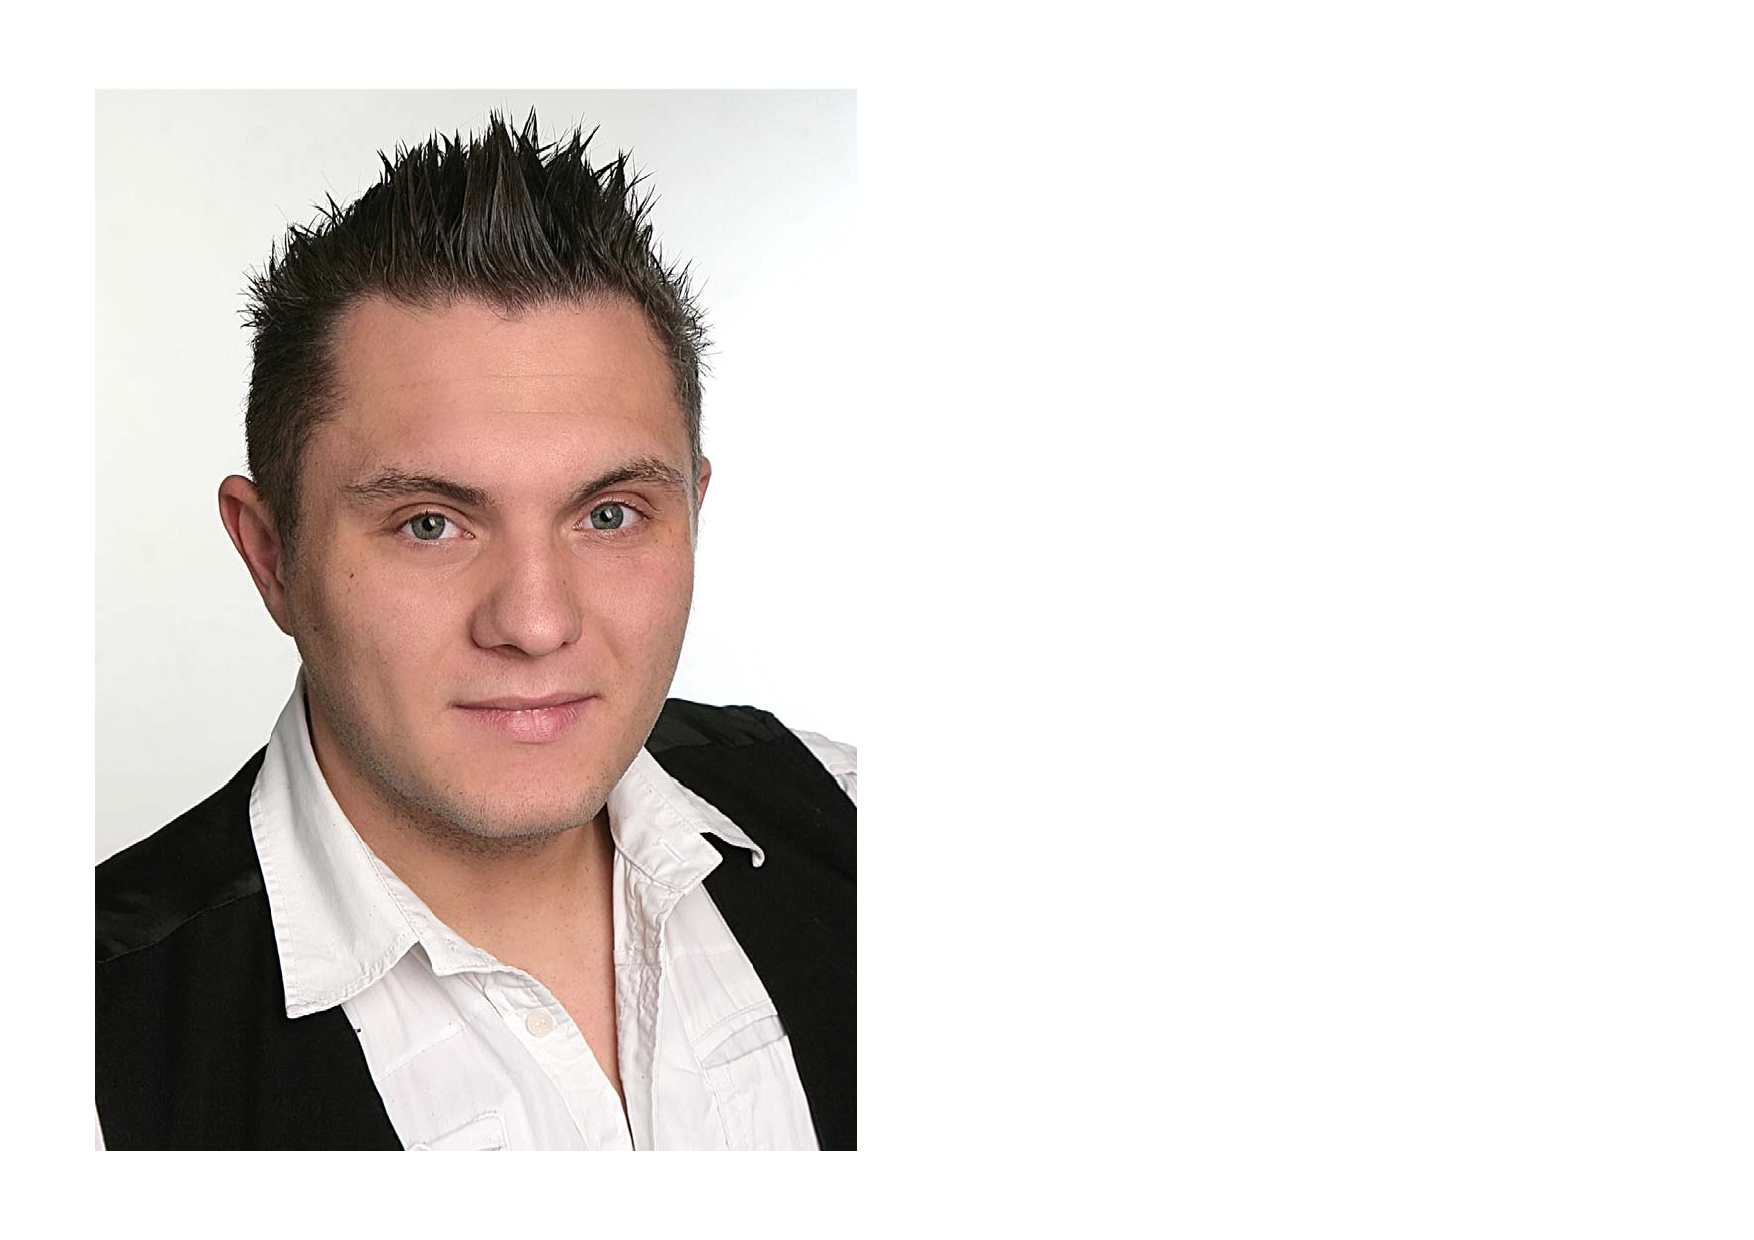
\includegraphics[width=1in,height=1.25in,clip,keepaspectratio]{BT.pdf}}]{Benjamin Ternes}\blindtext \end{biography}%
% or if you just want to reserve a space for a photo:

%\begin{IEEEbiography}[{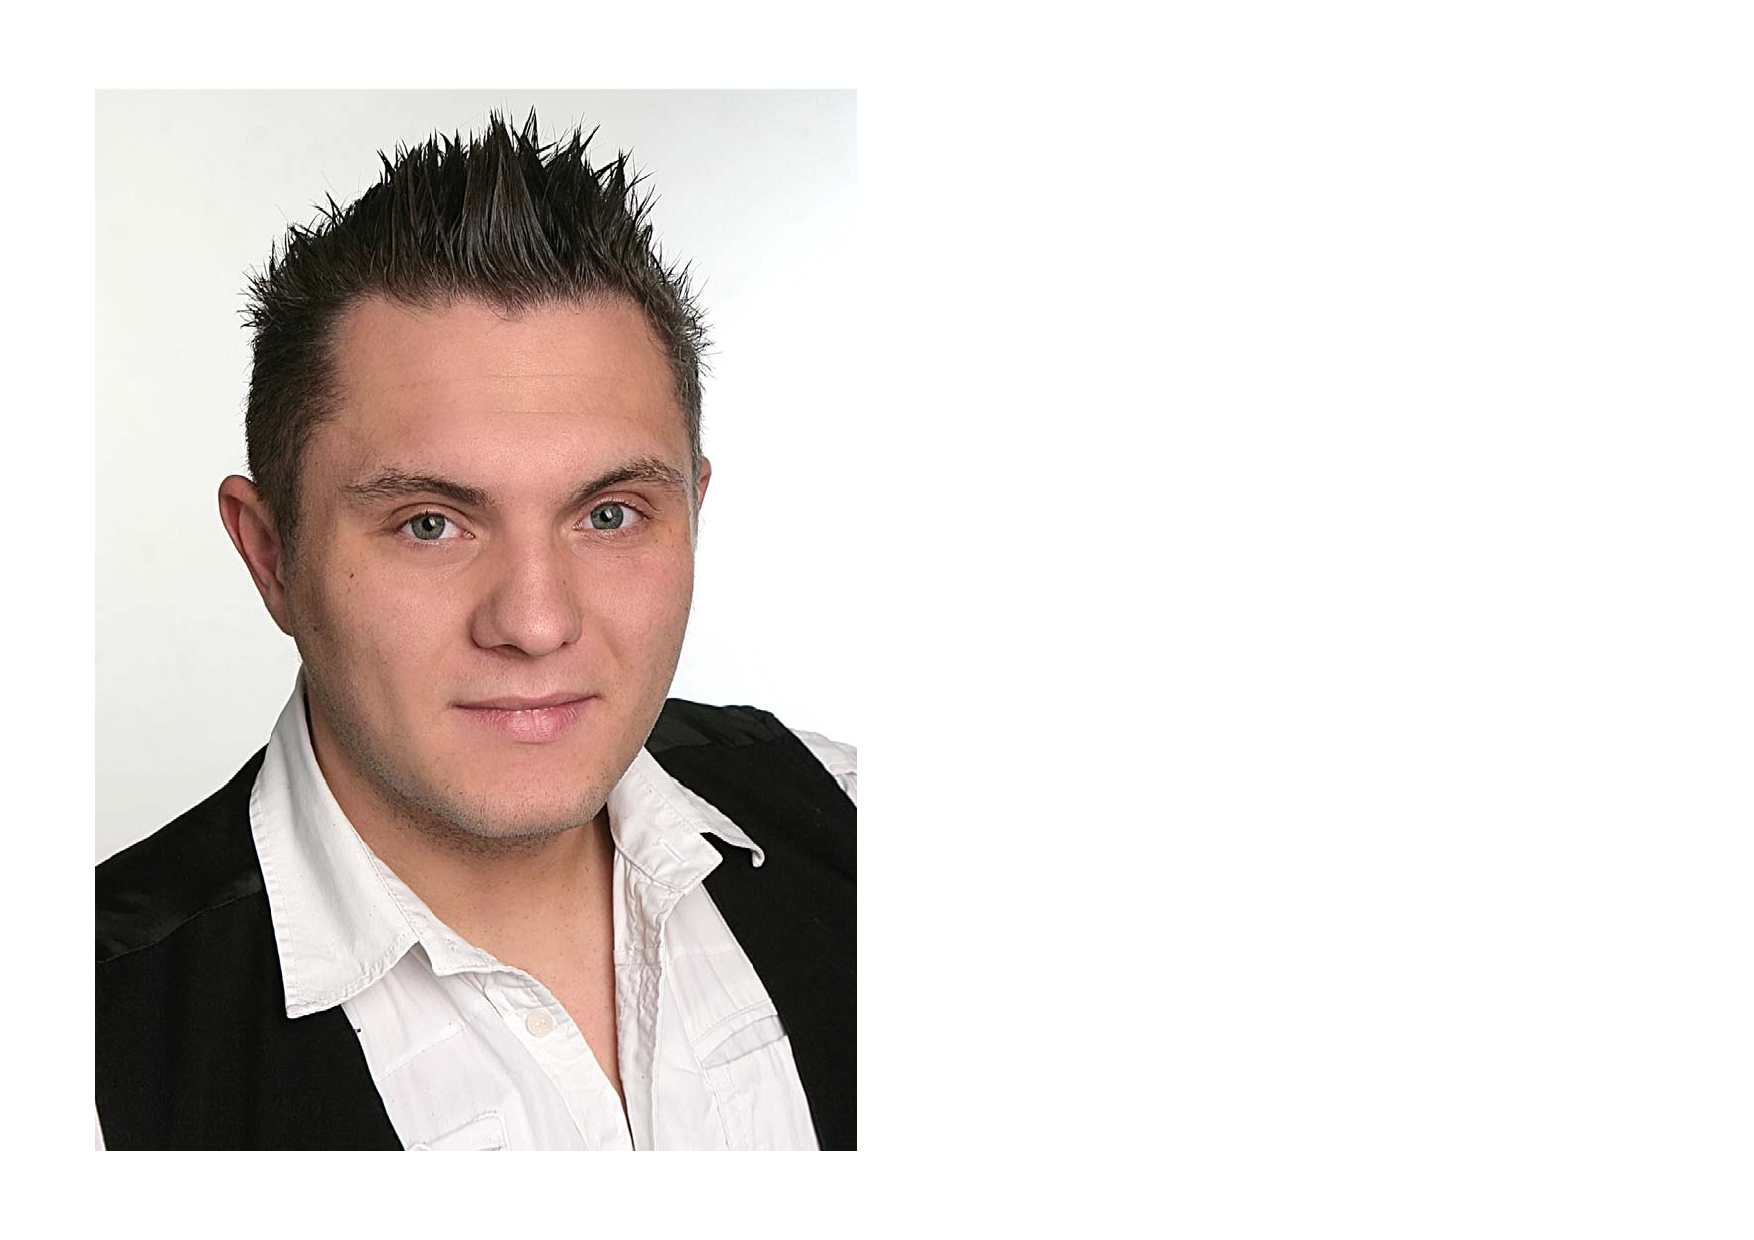
\includegraphics[width=1in,height=1.25in,clip,keepaspectratio]{BT.pdf}}]{Benjamin Ternes}
%studierte Elektrotechnik mit dem Schwerpunkt: Antriebs- und Automatisierungstechnik an der FH Dortmund, wo Herr Ternes auch den Abschluss Bachelor of Engineering erlangte. Derzeit ist Herr Ternes an der Hochschule Bochum als Master of Science (Elektrotechnik) eingeschrieben. Seine Forschungsschwerpunkte sind elektrische Maschinen, Systemtheorie und Identifikationsverfahren zur Bestimmung von Maschinenparametern. Nebenbei arbeitet Herr Ternes an der FernUniversität in Hagen als WHF.
%\end{IEEEbiography}
% You can push biographies down or up by placing
% a \vfill before or after them. The appropriate
% use of \vfill depends on what kind of text is
% on the last page and whether or not the columns
% are being equalized.

%\vfill

% Can be used to pull up biographies so that the bottom of the last one
% is flush with the other column.
%\enlargethispage{-5in}




% that's all folks
\end{document}


